\textbf{📋 Apa yang akan dipelajari}

Pada bab ini kita akan mempelajari dasar-dasar yang perlu diketahui sebelum mulai belajar C++ dan Qt:

\begin{itemize}
\item Sejarah dan pengenalan bahasa C++
\item Keunggulan bahasa C++ dibanding bahasa lain
\item Pengenalan Qt Creator dan fitur-fiturnya
\item Teknologi UI Qt (Widget, Quick, WebKit)
\item Cara instalasi Qt Creator di berbagai platform
\item Membuat program pertama "Hello World"
\item Struktur dasar program C++
\end{itemize}

\minitoc

\section{🌍 Sejarah Bahasa C++}

\subsection{Awal Mula Bahasa C}

Bahasa C adalah bahasa pemrograman yang dibuat pada tahun 1972 oleh \textbf{Dennis M. Ritchie} di Bell Laboratories. Bahasa ini dirancang sebagai bahasa pemrograman tingkat menengah - tidak terlalu rumit seperti bahasa assembly, tapi juga tidak terlalu sederhana seperti bahasa tingkat tinggi.

\begin{center}
\begin{tabular}{|l|l|}
\hline
\textbf{Tahun} & \textbf{Peristiwa} \\
\hline
1972 & Dennis Ritchie menciptakan bahasa C \\
\hline
1978 & Buku "The C Programming Language" diterbitkan \\
\hline
1989 & Bahasa C distandarisasi oleh ANSI \\
\hline
\end{tabular}
\end{center}

\subsection{Kelahiran Bahasa C++}

Bahasa C++ adalah pengembangan dari bahasa C yang dibuat oleh \textbf{Bjarne Stroustrup} di Bell Labs. Nama "C++" berasal dari operator increment "++" dalam C, yang berarti "C yang ditingkatkan".

\begin{quote}
\textit{"C++ adalah bahasa pemrograman yang dirancang untuk mendukung pemrograman berorientasi objek sambil tetap mempertahankan efisiensi dan fleksibilitas bahasa C."} - Bjarne Stroustrup
\end{quote}

\subsection{Perkembangan Bahasa C++}

Bahasa C++ mengalami evolusi yang signifikan:

\begin{enumerate}
\item \textbf{1985:} AT\&T Laboratories merilis \textbf{cfront} - kompiler C++ pertama
\item \textbf{1990:} Borland International mengembangkan kompiler C++ langsung
\item \textbf{1998:} Standar C++ pertama (C++98)
\item \textbf{2003:} Standar C++03 (perbaikan minor)
\item \textbf{2011:} Standar C++11 (modernisasi besar)
\item \textbf{2014:} Standar C++14 (perbaikan C++11)
\item \textbf{2017:} Standar C++17 (fitur baru)
\item \textbf{2020:} Standar C++20 (fitur modern)
\end{enumerate}

\section{⭐ Keunggulan Bahasa C++}

Berikut adalah keunggulan-keunggulan bahasa C++ dibandingkan bahasa pemrograman lainnya:

\begin{description}

\item[🎯 \textbf{Pemrograman Berorientasi Objek (OOP)}]
C++ mendukung pemrograman berorientasi objek yang memungkinkan kita melihat masalah sebagai objek-objek yang saling berinteraksi, bukan sebagai prosedur-prosedur yang berurutan.

\begin{itemize}
\item \textbf{Encapsulation} - Penggabungan data dan fungsi
\item \textbf{Inheritance} - Pewarisan sifat dari class lain
\item \textbf{Polymorphism} - Kemampuan objek berperilaku berbeda
\end{itemize}

\item[🌍 \textbf{Portabilitas}]
Kode C++ yang sama bisa dikompilasi dan dijalankan di berbagai jenis komputer dan sistem operasi tanpa perubahan.

\begin{itemize}
\item \textbf{Cross-platform} - Windows, Linux, macOS
\item \textbf{Standard library} - Konsisten di semua platform
\item \textbf{Compiler support} - Didukung semua compiler utama
\end{itemize}

\item[⚡ \textbf{Kecepatan dan Efisiensi}]
C++ memberikan kontrol penuh atas memory dan resources.

\begin{itemize}
\item \textbf{Direct memory access} - Akses langsung ke memory
\item \textbf{No garbage collection} - Tidak ada overhead GC
\item \textbf{Optimized compilation} - Kode yang sangat efisien
\end{itemize}

\item[🔧 \textbf{Pemrograman Modular}]
Program C++ bisa terdiri dari beberapa file yang terpisah dan kemudian digabungkan.

\begin{itemize}
\item \textbf{Header files} - Deklarasi fungsi dan class
\item \textbf{Source files} - Implementasi fungsi dan class
\item \textbf{Libraries} - Kode yang bisa digunakan ulang
\end{itemize}

\item[🔄 \textbf{Kompatibilitas dengan C}]
C++ sangat kompatibel dengan bahasa C. Kode program yang ditulis dalam C bisa digabungkan dengan C++ dengan mudah.

\begin{itemize}
\item \textbf{C functions} - Bisa dipanggil dari C++
\item \textbf{C libraries} - Bisa digunakan di C++
\item \textbf{Gradual migration} - Migrasi bertahap dari C ke C++
\end{itemize}

\item[📝 \textbf{Keringkasan dan Fleksibilitas}]
C++ adalah bahasa tingkat tinggi yang ringkas dan fleksibel.

\begin{itemize}
\item \textbf{Multiple paradigms} - OOP, procedural, generic
\item \textbf{Operator overloading} - Operator bisa didefinisikan ulang
\item \textbf{Templates} - Kode generik yang efisien
\end{itemize}

\end{description}

\section{🛠️ Pengenalan Qt Creator}

\subsection{Apa itu Qt Creator?}

Qt Creator adalah \textbf{Integrated Development Environment (IDE)} untuk bahasa C++ yang bisa digunakan di berbagai sistem operasi (cross-platform). IDE adalah program yang menyediakan semua tools yang diperlukan untuk menulis, mengkompilasi, dan menjalankan program dalam satu aplikasi.

\begin{quote}
\textit{Qt Creator adalah IDE yang powerful dan user-friendly yang dirancang khusus untuk pengembangan aplikasi Qt.}
\end{quote}

\subsection{Fitur Utama Qt Creator}

\begin{itemize}
\item \textbf{Code Editor} - Editor kode dengan syntax highlighting dan autocompletion
\item \textbf{Visual Designer} - Designer GUI untuk membuat antarmuka pengguna
\item \textbf{Debugger} - Debugger visual untuk mencari dan memperbaiki bug
\item \textbf{Project Manager} - Manajemen project yang terintegrasi
\item \textbf{Version Control} - Dukungan Git, SVN, dan lainnya
\item \textbf{Cross-platform} - Sama di Windows, Linux, macOS
\end{itemize}

\subsection{Kompiler yang Didukung}

Qt Creator bisa menggunakan berbagai kompiler C++:

\begin{center}
\begin{tabular}{|l|l|l|}
\hline
\textbf{Kompiler} & \textbf{Platform} & \textbf{Keunggulan} \\
\hline
MinGW & Windows & Gratis, ringan \\
\hline
MSVC & Windows & Terintegrasi dengan Visual Studio \\
\hline
GCC & Linux/macOS & Standar, powerful \\
\hline
Clang & Multi-platform & Modern, cepat \\
\hline
\end{tabular}
\end{center}

\subsection{Format Project Qt Creator}

Qt Creator menggunakan format project \textbf{cross-platform} (.pro) yang memungkinkan tim developer berbagi project di berbagai platform yang berbeda.

\begin{itemize}
\item \textbf{File .pro} - Konfigurasi project
\item \textbf{Source files} - File .cpp dan .h
\item \textbf{UI files} - File .ui untuk GUI
\item \textbf{Resource files} - File .qrc untuk resources
\item \textbf{Build settings} - Konfigurasi kompilasi
\end{itemize}

\subsection{Cara Membuat Project}

Project bisa dibuat dengan dua cara:
\begin{itemize}
\item \textbf{Manual} - Qt Creator akan menghasilkan file-file yang diperlukan secara otomatis
\item \textbf{Import} - Menggunakan project yang sudah ada
\end{itemize}

\begin{figure}[htbp]
\centering 
\shadowimage[width=8cm]{Capture1-1}
\caption{Projek pada Qt Creator}
\label{fig:projek-pada-qt-creator}
\end{figure}

\subsection{Code Editor Qt Creator}

Editor kode Qt Creator terintegrasi dengan Qt Designer untuk membuat aplikasi GUI. Qt Creator memisahkan antara editor untuk menulis kode dan editor untuk menjalankan aplikasi.

\begin{figure}[htbp]
\centering
\shadowimage[width=8cm]{Capture1-2}
\label{fig:code-editor}
\caption{Code Editor Qt Creator}
\end{figure}

\subsection{Keunggulan Code Editor}

\begin{enumerate}
\item \textbf{Syntax Highlighting} - Warna berbeda untuk keyword, string, comment
\item \textbf{Code Completion} - Menebak dan melengkapi kode yang akan ditulis
\item \textbf{Error Detection} - Menampilkan error dan warning secara real-time
\item \textbf{Code Navigation} - Jump to definition, find references
\item \textbf{Refactoring} - Rename, extract method, move class
\item \textbf{Code Formatting} - Format kode secara otomatis
\item \textbf{Integrated Help} - Dokumentasi yang terintegrasi
\end{enumerate}

\subsection{UI Designer}

Qt Creator menyajikan dua buah editor visual: \textbf{Qt Designer} dan \textbf{Qt Quick Designer}.

\subsubsection{Qt Designer}

Qt Designer adalah tool untuk mendesain dan membangun aplikasi GUI dari Qt widgets. Widgets dan forms yang dibentuk dengan Qt Designer terintegrasi dengan code program, Qt signals dan mekanisme slots.

\begin{itemize}
\item \textbf{Drag and Drop} - Seret komponen ke form
\item \textbf{Property Editor} - Edit properti komponen
\item \textbf{Signal/Slot Editor} - Hubungkan signal dan slot
\item \textbf{Layout Management} - Atur layout secara visual
\end{itemize}

\subsubsection{Qt Quick Designer}

Qt Quick Designer digunakan untuk membangun animasi-animasi dengan menggunakan QML (Qt Meta-Object Language). Dalam QML, sebuah user interface dispesifikasikan sebagai sebuah pohon (tree) dari objects dengan properti-properti.

\begin{figure}[htbp]
\centering
\shadowimage[width=8cm]{Capture1-3}
\caption{Gambar UI Designers}
\label{fig:gambar-ui-designers}
\end{figure}

\subsection{Bahasa yang Didukung}

Anda dapat menggunakan code editor untuk menulis kode dalam:
\begin{itemize}
\item \textbf{Qt C++} - Bahasa utama untuk Qt
\item \textbf{QML} - Qt Meta-Object Language
\item \textbf{JavaScript} - Untuk logika aplikasi
\item \textbf{HTML5} - Untuk konten web
\item \textbf{Python} - Dengan Qt for Python
\end{itemize}

\subsection{Platform yang Didukung}

Qt Creator mendukung untuk membangun dan menjalankan aplikasi Qt untuk:

\begin{itemize}
\item \textbf{Desktop} - Windows, Linux, FreeBSD, macOS
\item \textbf{Mobile} - Android, iOS, Windows Phone
\item \textbf{Embedded} - Linux embedded, QNX, VxWorks
\item \textbf{Web} - WebAssembly
\end{itemize}

\subsection{Tools Terintegrasi}

Qt Creator diintegrasikan dengan kumpulan tool-tool yang bermanfaat:

\begin{itemize}
\item \textbf{Version Control} - Git, SVN, Mercurial, CVS
\item \textbf{Qt Simulator} - Simulator untuk testing
\item \textbf{Qt Assistant} - Dokumentasi Qt
\item \textbf{Qt Linguist} - Tool untuk internationalization
\item \textbf{Qt Designer} - Visual GUI designer
\end{itemize}

\subsection{Debuggers}

Qt Creator mempunyai plugin debugger yang bekerja sebagai interface antara Qt Creator core dan external native debuggers:

\begin{itemize}
\item \textbf{GNU Symbolic Debugger (gdb)} - Debugger standar
\item \textbf{Microsoft Console Debugger (CDB)} - Untuk Windows
\item \textbf{LLDB} - Debugger modern dari LLVM
\item \textbf{JavaScript debugger} - Untuk QML dan JavaScript
\end{itemize}

\section{🎨 Teknologi User Interface (UI) Qt}

\subsection{Apa itu User Interface?}

User Interface (UI) adalah cara pengguna berinteraksi dengan program komputer. UI bisa berupa window, tombol, text area, dan komponen visual lainnya.

Qt menyediakan tiga teknologi UI yang bisa dipilih sesuai kebutuhan:
\begin{itemize}
\item \textbf{QtWidget} - UI tradisional untuk desktop
\item \textbf{QtQuick} - UI modern dengan animasi
\item \textbf{QtWebKit} - UI berbasis web
\end{itemize}

\subsection{Contoh Penggunaan di Qt Creator}

Qt Creator sendiri adalah contoh bagus dari penggunaan multiple teknologi UI:

\begin{itemize}
\item \textbf{Menu dan dialog} menggunakan QtWidget
\item \textbf{Welcome Screen} menggunakan QtQuick (tampilan modern dengan animasi)
\item \textbf{Help Documentation} menggunakan QtWebKit (seperti halaman web)
\end{itemize}

Anda bisa menggabungkan ketiga teknologi ini dalam satu aplikasi! 😊

\subsection{🚀 QtQuick - UI Modern dengan Animasi}

QtQuick adalah teknologi UI modern Qt yang menggunakan \textbf{QML} (Qt Meta-Object Language) dan \textbf{JavaScript} untuk membuat antarmuka pengguna.

\subsubsection{Fitur QtQuick}

\begin{itemize}
\item \textbf{Animasi dan transisi} yang halus
\item \textbf{Visual effects} yang menarik
\item \textbf{Hardware acceleration} menggunakan OpenGL
\item \textbf{Responsive design} yang mudah
\item \textbf{Touch support} untuk perangkat mobile
\end{itemize}

\subsubsection{Keuntungan QtQuick}

\begin{itemize}
\item Cocok untuk aplikasi modern dengan animasi
\item Performa tinggi dengan hardware acceleration
\item Mudah membuat UI yang menarik
\item Mendukung touch dan gesture
\item Cross-platform untuk desktop dan mobile
\end{itemize}

\subsubsection{Perlu Diperhatikan}

QtQuick membutuhkan dukungan OpenGL dari kartu grafis. Jika OpenGL tidak tersedia, Anda perlu menginstal driver VGA yang sesuai dengan motherboard Anda.

\subsection{🖥️ QtWidget - UI Tradisional Desktop}

QtWidget adalah teknologi UI tradisional Qt yang menyediakan komponen-komponen standar untuk aplikasi desktop seperti button, text area, menu, dan lainnya.

\subsubsection{Karakteristik QtWidget}

\begin{itemize}
\item \textbf{UI tradisional} yang familiar dengan pengguna desktop
\item \textbf{Menyesuaikan dengan OS} - tampilan mirip dengan sistem operasi
\item \textbf{Komponen standar} yang sudah dikenal
\item \textbf{Cocok untuk aplikasi bisnis} dan aplikasi tradisional
\item \textbf{Stable dan mature} - teknologi yang sudah lama ada
\end{itemize}

\subsubsection{Base Class QtWidget}

Saat membuat aplikasi QtWidget, Anda akan diminta memilih Base Class:

\begin{enumerate}
\item \textbf{QWidget} - Base class untuk semua elemen GUI QtWidget
\item \textbf{QDialog} - Window dialog untuk input atau konfirmasi
\item \textbf{QMainWindow} - Window utama dengan menu bar, toolbar, dan status bar built-in
\end{enumerate}

\subsubsection{Kapan Menggunakan QtWidget}

\begin{itemize}
\item Aplikasi desktop tradisional
\item Aplikasi bisnis atau enterprise
\item Ketika ingin tampilan yang familiar dengan OS
\item Aplikasi yang tidak memerlukan animasi kompleks
\item Aplikasi yang membutuhkan stabilitas tinggi
\end{itemize}

\subsection{🌐 QtWebKit - UI Berbasis Web}

QtWebKit memungkinkan Anda membuat aplikasi desktop menggunakan teknologi web seperti HTML, CSS, dan JavaScript.

\subsubsection{Konsep QtWebKit}

\begin{itemize}
\item \textbf{Web content} ditampilkan melalui QML
\item \textbf{C++ API} digunakan untuk interaksi dengan konten web
\item \textbf{HTML5 dan CSS3} untuk tampilan modern
\item \textbf{JavaScript} untuk logika aplikasi
\end{itemize}

\subsubsection{Keuntungan QtWebKit}

\begin{itemize}
\item \textbf{Menggunakan skill web} yang sudah ada
\item \textbf{HTML5 dan CSS3} untuk tampilan modern
\item \textbf{JavaScript} yang mudah dipelajari
\item \textbf{Kompatibilitas web} yang luas
\item \textbf{Rapid prototyping} - cepat membuat prototype
\end{itemize}

\subsubsection{Kapan Menggunakan QtWebKit}

\begin{itemize}
\item Aplikasi yang membutuhkan konten web
\item Developer yang sudah familiar dengan HTML/CSS/JavaScript
\item Aplikasi yang perlu menampilkan halaman web
\item Prototype cepat dengan teknologi web
\item Aplikasi hybrid web-desktop
\end{itemize}

\subsection{📊 Perbandingan Teknologi UI Qt}

\begin{center}
\begin{tabular}{|l|l|l|l|}
\hline
\textbf{Fitur} & \textbf{QtWidget} & \textbf{QtQuick} & \textbf{QtWebKit} \\
\hline
Tampilan & Tradisional & Modern & Web-based \\
\hline
Animasi & Terbatas & Lengkap & CSS3 \\
\hline
Kemudahan & Mudah & Menengah & Mudah \\
\hline
Performa & Cepat & Sangat Cepat & Sedang \\
\hline
Platform & Desktop & Multi-platform & Multi-platform \\
\hline
Learning Curve & Rendah & Sedang & Rendah \\
\hline
\end{tabular}
\end{center}

\section{📥 Install Qt Creator}

Pada tutorial ini kita akan menginstall Qt Creator di berbagai platform. Qt Creator dapat diunduh di \href{http://www.qt.io/download}{halaman resmi Qt}\footnote{https://www.qt.io/download-open-source/\#section-2}.

\begin{figure}[htbp]
\centering
\shadowimage[width=8cm]{qt-downloads}
\label{halaman-web-download-qt}
\caption{Halaman web Download Qt Creator}
\end{figure}

\subsection{Install Qt Creator di Ubuntu/Linux}

\subsubsection{Langkah 1: Download}

Kunjungi website Qt untuk mendownload Qt Creator sesuai dengan versi sistem operasi yang digunakan (64-bit atau 32-bit). Atau download menggunakan command line:

\begin{lstlisting}[language=sh]{../code/01-pengenalan-code-1.sh}
\end{lstlisting}

Untuk sistem 64-bit:
\begin{lstlisting}[language=sh]{../code/01-pengenalan-code-2.sh}
\end{lstlisting}

\subsubsection{Langkah 2: Install}

Atur permission, jalankan installer dan ikuti perintah berikut untuk menginstall Qt Creator secara lengkap:

\begin{lstlisting}[language=sh]{../code/01-pengenalan-code-3.sh}
\end{lstlisting}

\subsubsection{Langkah 3: Install g++}

Buka terminal untuk menginstal g++:

\begin{lstlisting}[language=sh]{../code/01-pengenalan-code-4.sh}
\end{lstlisting}

\subsubsection{Langkah 4: Konfigurasi Kompiler}

Buka Qt Creator, klik Tools → Options. Klik Build \& Run dan pilih tab Kit. Konfigurasikan kompiler jika belum terdeteksi secara otomatis.

\subsubsection{Langkah 5: Install Pustaka OpenGL}

Jalankan perintah berikut untuk menginstall Pustaka OpenGL:

\begin{lstlisting}[language=sh]{../code/01-pengenalan-code-5.sh}
\end{lstlisting}

\subsection{Install Qt Creator di Windows}

\subsubsection{Langkah 1: Download}

Anda dapat mendownload Qt Creator di halaman website Qt dan memilih versi yang sesuai dengan sistem operasi Anda (64-bit atau 32-bit).
 
\begin{center}
	 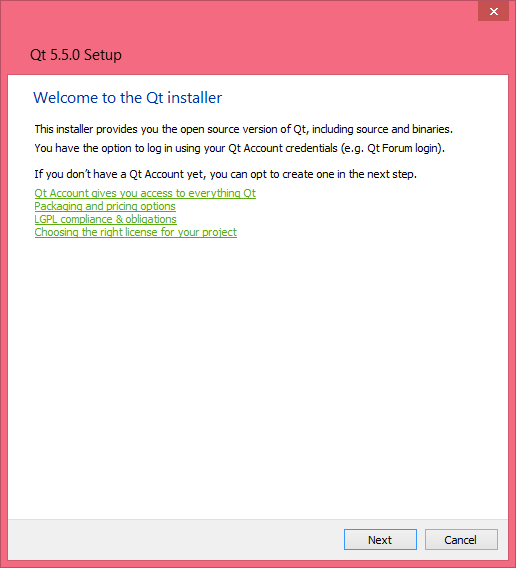
\includegraphics[width=0.4\textwidth]{install-qt-1}
\end{center}
 
\subsubsection{Langkah 2: Install}

Jika Anda telah mendownload Qt Creator, jalankan installer. Pilih versi yang sesuai dengan sistem operasi Anda.

\begin{center}
	 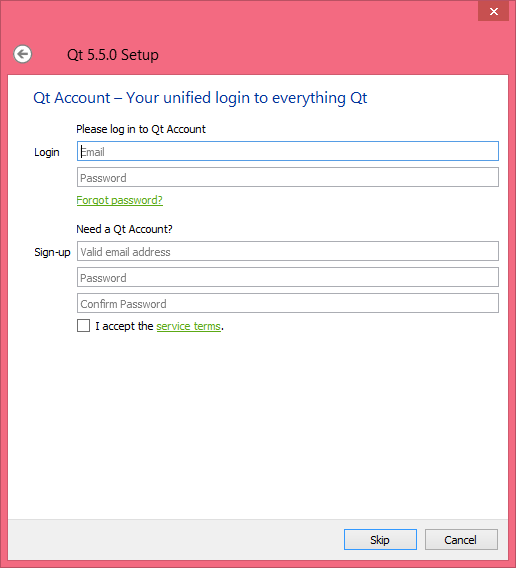
\includegraphics[width=0.4\textwidth]{install-qt-2}
\end{center}
 
\subsubsection{Langkah 3: Setup}
  
Pilih "Next" dan ikuti langkah-langkah setup. Jika tidak ingin mendaftar, Anda dapat memilih "Skip".
  
\begin{center}
	 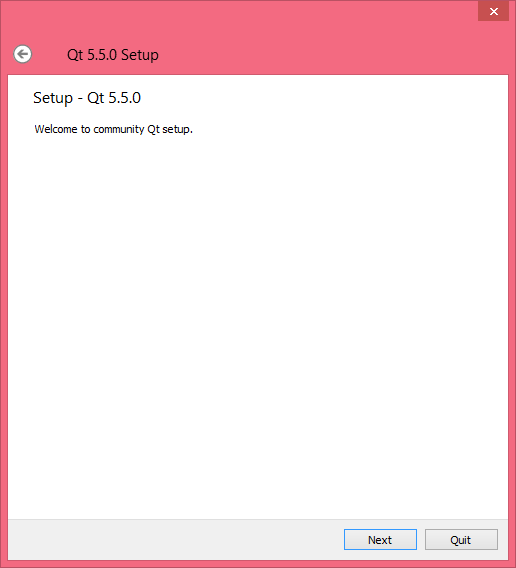
\includegraphics[width=0.4\textwidth]{install-qt-3}
\end{center}
 
\subsubsection{Langkah 4: Selesai}

Installer akan menginstall aplikasi sampai selesai. Klik "Finish" untuk mengakhiri proses pemasangan.

\begin{center}
	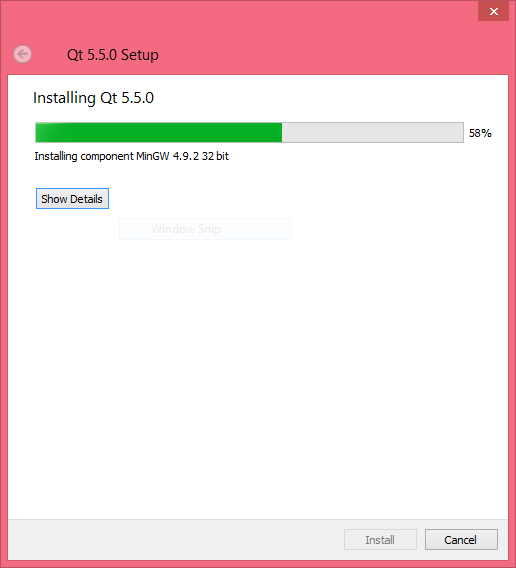
\includegraphics[width=0.4\textwidth]{install-qt-4}
\end{center}

\section{🚀 Program Console Pertama dengan Qt Creator}

\subsection{Membuat Project Console}

Untuk mencoba membuat aplikasi dengan Qt Creator, ikuti langkah-langkah berikut:

\begin{enumerate}
\item Buka Qt Creator
\item Klik File → New Project
\item Pilih Application → Qt Console Application
\item Klik "Choose"
\end{enumerate}

  \begin{center}
  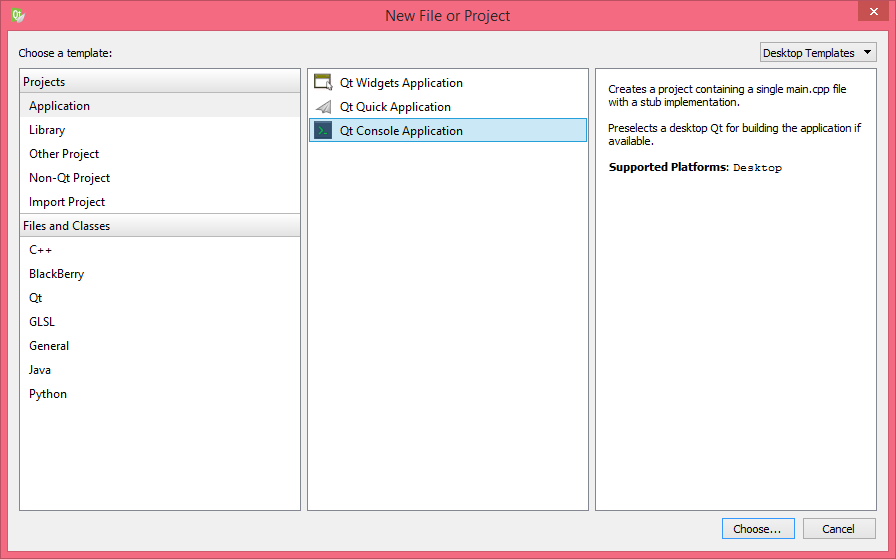
\includegraphics[width=0.8\textwidth]{qt-console-aplication}
  \end{center}

\subsection{Konfigurasi Project}

Beri nama project dan pilih direktori tempat aplikasi akan disimpan:

  \begin{center}
  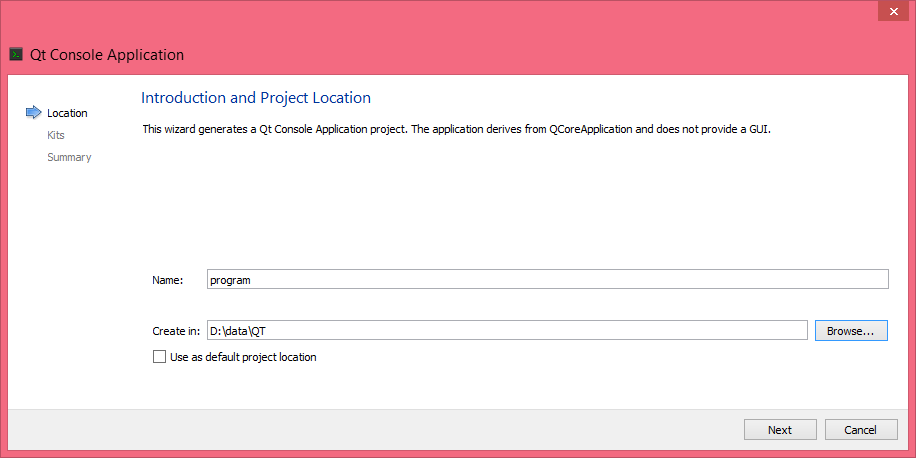
\includegraphics[width=0.8\textwidth]{qt-console-aplication-2}
  \end{center}

\subsection{Pilih Kompiler}

Klik "Next", kemudian pilih kompiler yang akan digunakan. Disini penulis menggunakan MinGW sebagai kompilernya.

\begin{quotation}
{\LARGE \ding{46}} \textbf{Tips}

Simulator atau kompiler yang tersedia:
\begin{itemize}
\item Qt Simulator MinGW 4.4
\item Qt Simulator VS 2008, 2010, 2011, 2012, 2013, 2014
\item Android SDK dan NDK
\end{itemize}
\end{quotation}

\begin{center}
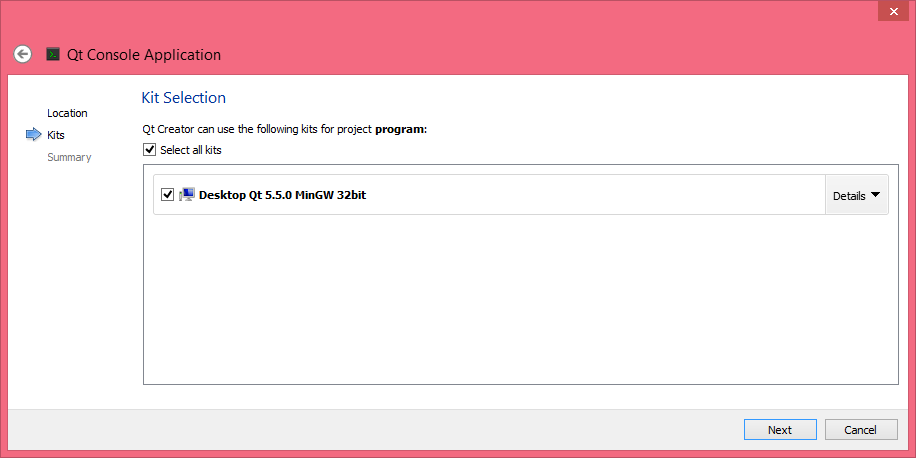
\includegraphics[width=0.8\textwidth]{qt-console-aplication-3}
\end{center}

\subsection{Version Control}

Pilih jenis version control yang akan digunakan. Jika Anda tidak menggunakan version control, pilih "None" pada "Add to version control".

\begin{figure}[htbp]
\centering
\shadowimage[width=8cm]{qt-console-aplication-4}
\caption{Langkah Setup Qt Creator}
\end{figure}

\subsection{Hasil Akhir}

Apabila dilakukan dengan benar, akan muncul Qt Editor seperti berikut:

\begin{center}
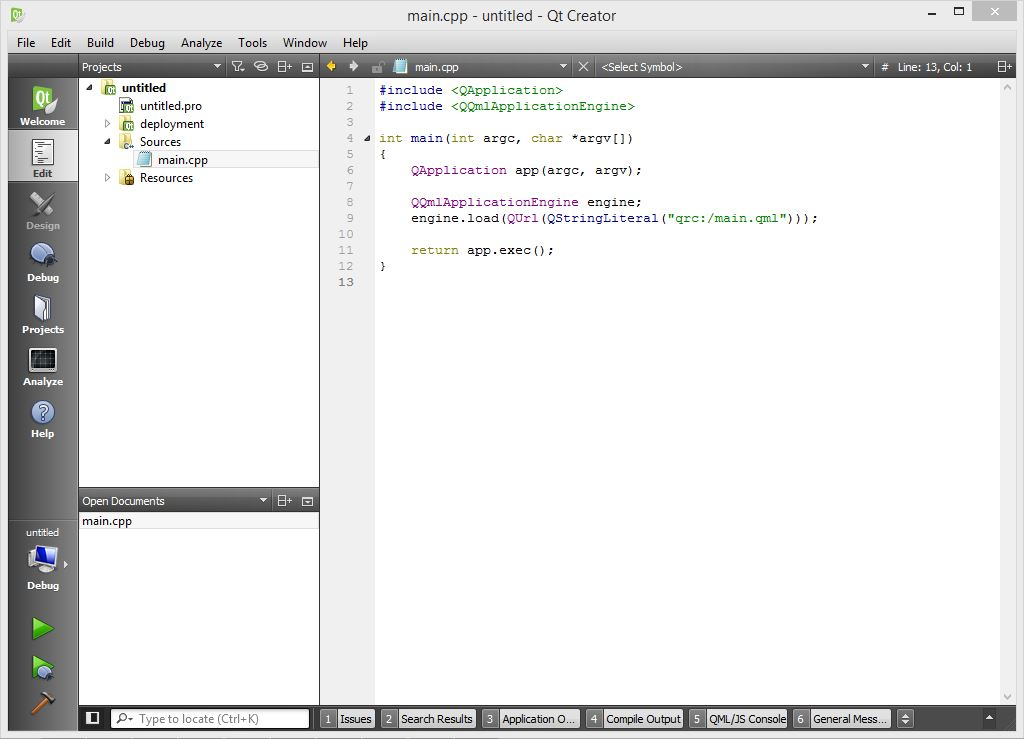
\includegraphics[width=0.8\textwidth]{qt-creator}
\end{center}

\section{📝 Struktur Program C++}

\subsection{Pengenalan Struktur Program}

Program Bahasa C/C++ tidak mengenal aturan penulisan di kolom/baris tertentu, jadi bisa dimulai dari kolom/baris manapun. Namun demikian, untuk mempermudah pembacaan program dan untuk keperluan dokumentasi, sebaiknya penulisan program di bahasa C/C++ diatur sedemikian rupa sehingga mudah dan enak dibaca.

\subsection{Struktur Dasar Program C++}

Berikut adalah struktur dasar program yang dibuat dengan bahasa C++:

\begin{lstlisting}[language=c++, caption=Struktur Program C++]
#include <header>  
using namespace std;    
int main(int argc, char *argv[])
{  
deklarasi variabel;   
deklarasi konstanta;  
perintah perintah;  
//komentar  
return 0;  
}  
\end{lstlisting}

\subsection{Penjelasan Komponen}

\subsubsection{1. \#include <header>}

\texttt{\#include} adalah salah satu pengarah preprocessor directive yang tersedia pada C++. Preprocessor selalu dijalankan terlebih dahulu pada saat proses kompilasi terjadi.

\begin{lstlisting}[language=c++]{../code/01-pengenalan-code-7.c++}
\end{lstlisting}

Bagian tersebut tidak diakhiri dengan tanda semicolon, karena bentuk tersebut bukanlah suatu bentuk pernyataan, tetapi merupakan preprocessor directive.

\subsubsection{Header Files yang Umum}

\begin{itemize}
\item \texttt{\#include <iostream>} - Input/output stream (cout, cin)
\item \texttt{\#include <conio.h>} - Console I/O (clrscr(), getch())
\item \texttt{\#include <iomanip>} - Input/output manipulators (setw())
\item \texttt{\#include <math.h>} - Mathematical functions (sqrt(), pow())
\item \texttt{\#include <string>} - String handling
\item \texttt{\#include <vector>} - Dynamic arrays
\item \texttt{\#include <algorithm>} - Standard algorithms
\end{itemize}

\subsubsection{2. using namespace std;}

Semua elemen standard C++ library dinyatakan dalam namespace bernama \texttt{std}. Dengan menulis \texttt{using namespace std;}, kita memberitahu compiler bahwa kita akan menggunakan semua elemen dari namespace std.

\begin{itemize}
\item \textbf{Namespace} - Cara mengelompokkan fungsi dan class
\item \textbf{std} - Standard namespace untuk C++ library
\item \textbf{using} - Memberitahu compiler namespace yang digunakan
\end{itemize}

\subsubsection{3. int main()}

Program C++ terdiri dari satu atau lebih fungsi, dan di antara salah satunya harus ada fungsi main dan hanya boleh ada satu main pada tiap program C++. Setiap program C++ akan dan pasti akan memulai eksekusi programnya pada fungsi main ini.

\begin{itemize}
\item \textbf{Entry point} - Titik masuk program
\item \textbf{Return type} - int (integer)
\item \textbf{Parameters} - argc (argument count), argv (argument vector)
\item \textbf{Curly braces} - \{ dan \} untuk scope
\end{itemize}

\subsubsection{4. Komentar}

Komentar tidak pernah dicompile oleh compiler. Dalam C++ terdapat 2 jenis komentar:

\begin{lstlisting}[language=c++, numbers=none]
  /* Komentar anda diletakkan
   di dalam ini bisa mengapit
    lebih dari satu baris */

  // Komentar anda diletakkan disini
// (hanya bisa sebaris)
\end{lstlisting}

\subsubsection{5. Tanda Semicolon (;)}

Tanda semicolon "\texttt{;}" digunakan untuk mengakhiri sebuah pernyataan. Setiap pernyataan harus diakhiri dengan sebuah tanda semicolon.

\begin{itemize}
\item \textbf{Statement terminator} - Mengakhiri pernyataan
\item \textbf{Required} - Wajib untuk setiap statement
\item \textbf{Common error} - Kesalahan yang sering terjadi
\end{itemize}

\subsubsection{6. return 0}

Pernyataan return menyebabkan fungsi utama untuk menyelesaikan kegiatannya lalu mengembalikan hasil dari fungsi utama.

\begin{itemize}
\item \textbf{return 0} - Program berakhir dengan sukses
\item \textbf{return 1} - Program berakhir dengan error
\item \textbf{Exit code} - Kode yang dikembalikan ke sistem operasi
\end{itemize}

\subsection{Contoh Program Lengkap}

Untuk lebih jelasnya, silakan coba ketik program berikut pada project baru:

\begin{lstlisting}[language=c++, caption=Struktur program C++]{../code/01-pengenalan-struktur-program-c.c++}
\end{lstlisting}

Kemudian jalankan dengan menekan tombol Run (CTRL + R)

\begin{lcverbatim}
Hello world
Selamat belajar C/C++ enter my world
\end{lcverbatim}

\subsection{Analisis Output}

\begin{itemize}
\item \textbf{Hello world} - Output dari cout pertama
\item \textbf{endl} - Memberikan newline (enter)
\item \textbf{Selamat belajar C/C++ enter my world} - Output dari cout kedua
\item \textbf{Tidak ada spasi} - Karena tidak ada spasi dalam string
\end{itemize}

\section{🎯 Best Practices untuk Pemula}

\subsection{Tips Menulis Kode}

\begin{enumerate}
\item \textbf{Gunakan indentasi yang konsisten} - 2 atau 4 spasi
\item \textbf{Tulis komentar yang jelas} - Jelaskan logika program
\item \textbf{Gunakan nama variabel yang bermakna} - Jangan gunakan a, b, c
\item \textbf{Test program secara teratur} - Jangan menulis semua kode sekaligus
\item \textbf{Gunakan version control} - Git untuk tracking perubahan
\end{enumerate}

\subsection{Kesalahan Umum Pemula}

\begin{itemize}
\item \textbf{Lupa semicolon} - Setiap statement harus diakhiri ;
\item \textbf{Salah nama header} - Perhatikan nama file header
\item \textbf{Lupa return 0} - Main function harus return nilai
\item \textbf{Salah case} - C++ case sensitive
\item \textbf{Lupa include} - Header yang diperlukan
\end{itemize}

\section{📚 Referensi dan Bacaan Lanjutan}

Untuk pemahaman yang lebih mendalam, pembaca dapat merujuk pada:

\begin{itemize}
\item \textbf{Qt Documentation} - Dokumentasi resmi Qt\footnote{Qt Company. (2023). "Qt Creator Manual". https://doc.qt.io/qtcreator/}
\item \textbf{C++ Reference} - Referensi lengkap C++\footnote{C++ Reference. (2023). "C++ Standard Library". https://en.cppreference.com/}
\item \textbf{Bjarne Stroustrup} - Pencipta C++\footnote{Stroustrup, B. (2013). "The C++ Programming Language Fourth Edition". Addison-Wesley.}
\item \textbf{Qt Tutorial} - Tutorial resmi Qt\footnote{Qt Company. (2023). "Qt Tutorials". https://doc.qt.io/qt-6/tutorials.html}
\end{itemize}

\section{🎉 Kesimpulan}

Pada bab ini kita telah mempelajari dasar-dasar C++ dan Qt Creator. Dengan memahami sejarah, keunggulan, dan cara menggunakan Qt Creator, Anda siap untuk mulai menulis program C++ yang lebih kompleks.

\begin{center}
\textbf{Selamat! Anda telah siap untuk belajar C++ dan Qt} 🚀
\end{center}

\vspace{1cm}

\begin{center}
\textit{--- Bab selanjutnya: Tipe Data dan Variabel ---}
\end{center}
